\documentclass[12pt,a4paper]{article}

\usepackage[left=1in,right=1in,top=1in,bottom=1in]{geometry}                % See geometry.pdf to learn the layout options. There are lots.
\usepackage[parfill]{parskip}    % Activate to begin paragraphs with an empty line rather than an indent
\usepackage{microtype} \hyphenpenalty=750
\usepackage{graphicx}
\usepackage{epstopdf} \DeclareGraphicsRule{.tif}{png}{.png}{`convert #1 `dirname #1`/`basename #1 .tif`.png}
% \usepackage[applemac]{inputenc}
\usepackage{booktabs}
% \usepackage{fancyhdr} \pagestyle{fancy} \chead{\hifibau} \cfoot{\thepage}
% \usepackage[english,ngerman]{babel}

\usepackage{siunitx}

\PassOptionsToPackage{hyphens}{url}\usepackage[colorlinks]{hyperref}
\usepackage{caption} \captionsetup{labelfont={sf,bf}, size=footnotesize}

\usepackage[superscript,biblabel]{cite}

% set format of document title
\usepackage{titling}
\pretitle{\begin{center}\Large\bfseries}
\posttitle{\end{center}\vspace{1em}}
\preauthor{\begin{center}\large}
\postauthor{\end{center}\vspace{1em}}
\predate{\begin{center}\large}
\postdate{\end{center}\vspace{1em}}

% set formats of section headings
\usepackage[explicit]{titlesec}
\titleformat{\title}{\centering}{\thesection.}{0.5em}{\MakeUppercase{#1}}
%\titleformat{\section}{\centering}{\thesection.}{0.5em}{\MakeUppercase{#1}}
\titleformat{\section}{}{\thesection.}{0.5em}{\MakeUppercase{#1}}
%\titleformat{\subsection}[runin]{\slshape}{\thesubsection.}{0.5em}{#1. }
\titleformat{\subsection}{\slshape}{\thesubsection.}{0.5em}{#1 }
\titleformat{\subsubsection}[runin]{\slshape}{\thesubsubsection.}{0.5em}{#1. }
 
\usepackage[T1]{fontenc} \usepackage[scaled=.90]{helvet} \renewcommand{\familydefault}{\sfdefault} \usepackage[helvet]{sfmath}

\newcommand{\Ohm}{\ensuremath{\Omega}}
\sisetup{detect-all} % tell siunitx to detect font stuff


% \setlength{\columnsep}{0.75cm} 

\graphicspath{{figures/}}

% \interfootnotelinepenalty=10000

\providecommand{\figr}[1]{Fig.~\ref{fig:#1}}
\providecommand{\figlabel}[1]{\label{fig:#1}}
\providecommand{\tabl}[1]{Tab.~\ref{tab:#1}}
\providecommand{\tablabel}[1]{\label{tab:#1}}
\providecommand{\secn}[1]{Sec.~\ref{sec:#1}}
\providecommand{\seclabel}[1]{\label{sec:#1}}


%% define formats of section and subsection etc. headings:
%    \makeatletter
%    \def\section{\@startsection{section}{1}%
%    \z@{.7\linespacing\@plus\linespacing}{.5\linespacing}%
%%    {\normalfont\bfseries\centering}}
%    {\Large\centering}}
%    
%    \def\subsection{\@startsection{subsection}{2}%
%    \z@{.5\linespacing\@plus.7\linespacing}{-.5em}%
%%    {\normalfont\bfseries\itshape}}
%    {\normalfont\itshape}}
%    
%    \def\subsubsection{\@startsection{subsubsection}{3}%
%    \z@{.5\linespacing\@plus.7\linespacing}{-.5em}%
%%    {\normalfont\bfseries}}
%    {\normalfont\itshape}}
%    
%    \makeatother



\title{The Open-Source Directly-Heated Triode \\ Electrostatic Headphone Amplifier \\ (OSDEHA)}
\author{Matthias Brennwald}
\date{THIS DOCUMENT IS UNDER CONSTRUCTION!\\ Draft Version \today}

\begin{document}

% \twocolumn[\maketitle]

\maketitle

\emph{Warning: This DIY project involves high voltage. Individuals utilizing the information provided must possess expert knowledge, adhere to stringent safety precautions, and assume full responsibility for all associated risks. The authors and contributors of this project expressly disclaim any liability for injuries or damages arising from the use or misuse of this information.}

\clearpage

\tableofcontents

\clearpage


\section{Overview}

This document describes an audio amplifier for electrostatic headphones. The design of the amplifier is targeted at DIY builders and is published as open hardware (see \secn{license}).

Electrostatic headphones operate on audio signals characterized by high voltage and low current. This is the domain of vacuum tubes, making them most suitable as drivers for electrostatic headphones.  While there exist a number of tube amplifiers for electrostatic headphones, many of these designs do not utilize directly-heated triodes (DHTs), which exhibit outstanding linearity and sound quality.\par

The OSDEHA uses DHT tubes for its output stage and implements the following design goals:
\begin{itemize}
\item The audio output is taken directly from the anodes of the DHT output tubes. There are no transformer or capacitors to transfer the power to the headphones.
\item The amplifier input takes balanced input at signal levels of modern audio sources (mostly DACs these days).
\item The design prioritizes the quality of audio reproduction and electronic design rather than on low cost.
\item The amplifier should be reasonably compact. The power supply unit may be a separate unit to keep the amplifier unit reasonable compact.
\end{itemize}

The OSDEHA design files, along with supporting documents and data, are available in the OSDEHA file repository\cite{osdeha_github}.

There is a public discussion thread of the OSDEHA at diyAudio\cite{osdeha_p1}. 


\section{Amplifier Design}

\subsection{Driving Electrostatic Headphones} \seclabel{estat_drive}

Electrostatic headphones operate using three electrodes: two fixed outer electrodes (stators) and a movable central electrode (diaphragm). The diaphragm is biased at a high voltage relative to the stators. The audio signal is applied to the stators in opposite polarities, generating an electric field that controls the movement of the charged diaphragm. For accurate sound reproduction, the electrostatic forces acting on the diaphragm must be proportional to the applied audio signal. To prevent distortion of the audio output, the charge on the diaphragm must remain constant.

The electrical impedance of electrostatic headphones is primarily determined by the capacitance of the two stators, which is typically around \SI{100}{pF}\cite{osdeha_p3}.

The voltage swing required to drive the stators depends on the headphone sensitivity and the desired sound pressure level. An experiment using various genres of well-recorded music indicated that an undistorted \SI{1.3}{kV} peak-to-peak swing of the bipolar output is desirable (i.e., \SI{650}{V} peak-to-peak at each stator)\cite{osdeha_p8}. The corresponding current swing measured in this experiment was approximately \SI{4}{mA}. However, driving the \SI{100}{pF} load to full output at frequencies up to \SI{20}{kHz} and beyond necessitates larger peak currents, around \SI{20}{mA}\cite{osdeha_p2}.


\subsection{Output Stage}\seclabel{outputstage}

\figr{OPS_concept} illustrates the conceptual layout of the OSDEHA. The output stage employs two DHTs in a push-pull configuration to deliver the symmetric, bipolar output required to drive electrostatic headphones. For efficient audio power transfer to the headphones, the AC impedance of the anode loads must be much larger that that of the headphones (several \unit{M\Ohm}). This cannot be achieved using passive anode-load resistors; instead, active constant-current sources (CCSs) are employed. The CCS loads not only enhance the amplifier's linearity and voltage gain but also suppress ripple and noise from the B+ rails.

\begin{figure}
\begin{center}
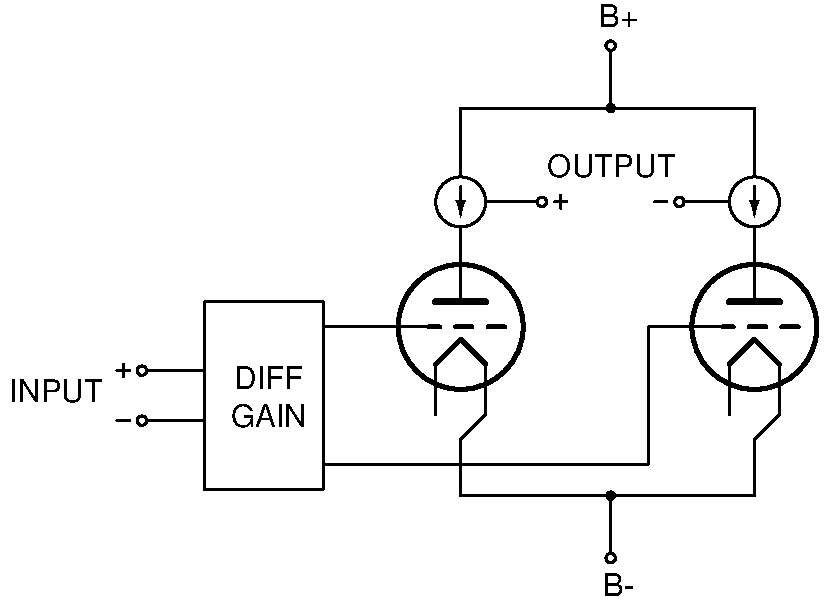
\includegraphics[width=0.7\textwidth]{OPS_concept.pdf}
\caption{Conceptual layout of the OSDEHA: differential input and gain stage, push-pull DHT output stage.}
\figlabel{OPS_concept}
\end{center}
\end{figure}

The choice of output tube type is dictated by the drive requirements of the headphones, as described in \secn{estat_drive}. Since the two tubes are connected in series with the headphones, each tube is responsible for half of the total voltage swing. Thus, each tube must handle a swing of \SI{\pm325}{V} at a \SI{20}{mA} bias. Furthermore, to emphasize the characteristic ``DHT sound,'' the DHT output stage should contribute as much voltage gain as possible to the overall amplifier gain.

Several DHT tube types were evaluated for the OSDEHA\cite{osdeha_p9,osdeha_whichDHT}. Specifically:

\begin{itemize}
\item The 841/VT-51 tube offers a gain of 30$\times$ and can be biased up to \SI{425}{V}. However, at the operating point required for the OSDEHA, the 841 tends to operate with a positive grid voltage, leading to grid current draw. Additionally, these tubes are relatively scarce.
\item The 20B tube is a modern design with a gain of 20$\times$ and supports biasing up to approximately \SI{500}{V}. However, these tubes are quite large (roughly the size of a beer bottle) and are produced only in small quantities by a single manufacturer (Emissionlabs), raising concerns about their long-term availability.
\item The family of the 801/801A/VT-62 and 10Y/VT-25 types\cite{aasyl_801types} provide a gain of 8$\times$. The 801 can be biased up to \SI{500}{V}, while the 10Y should not be biased above \SI{450}{V}. These tubes are available as new-old-stock and from new production.
\end{itemize}

From a technical perspective, the high gain of the 20B makes it an attractive option. However, due to concerns about the long-term availability of the 20B, the 801/10Y family of tubes is deemed a more practical choice for the OSDEHA design.

\figr{801A_curves} illustrates the characteristic curves measured from the 801A tube (with the 10Y/VT-25 being equivalent) along with the load line of a \SI{20}{mA} constant-current source (CCS). The anode DC bias is set to \SI{420}{V}, corresponding to a grid bias of approximately \SI{-34}{V}. This bias point allows for an anode voltage swing of \SI{\pm325}{V} within the tube's linear operating range. The grid voltage remains below +\SI{10}{V}, where measured grid current stays well under \SI{1}{mA}. With the anode voltage approaching ground potential, the B- voltage is set to \SI{-420}{V} and the B+ voltage to \SI{+420}{V}, maintaining symmetry.

\begin{figure}
\begin{center}
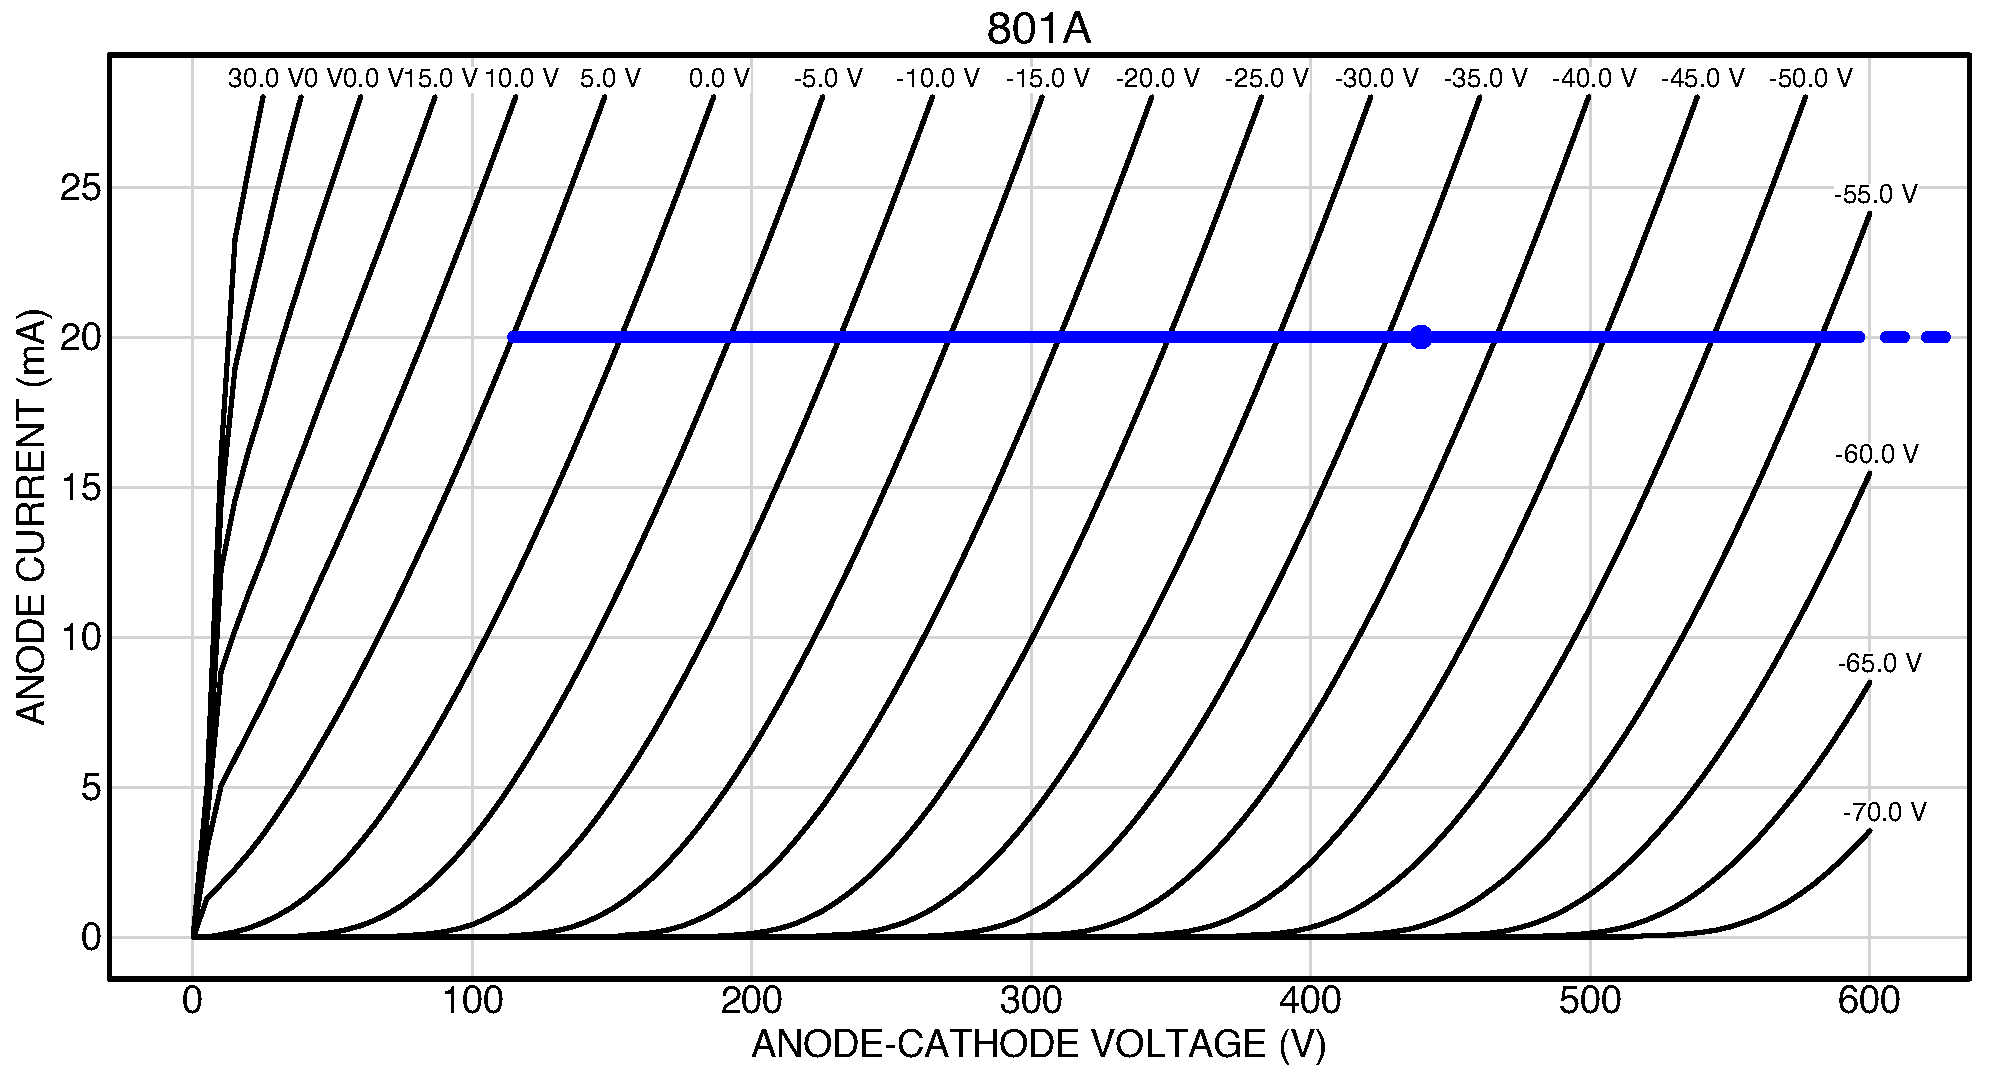
\includegraphics[width=0.8\textwidth]{801A_curves.pdf}
\caption{Characteristic curves of the 801A DHT, showing a DC bias point at \SI{420}{V} and \SI{20}{mA}, with a constant-current load line allowing an anode swing of \SI{\pm325}{V} (blue).}
\figlabel{801A_curves}
\end{center}
\end{figure}

\figr{activeload_concept} shows the simplified circuit of the CCSs used to load the anodes of the DHT output tubes. This circuit functions as a CCS in the audio/AC domain while providing a fixed voltage in the DC domain. In both cases, the FET Q1 controls the circuit's output to the anode. The depletion-mode FET Q2 drops most of the voltage from B+ and isolates Q1 from any noise or ripple present in the B+ supply.\par

\begin{figure}
\begin{center}
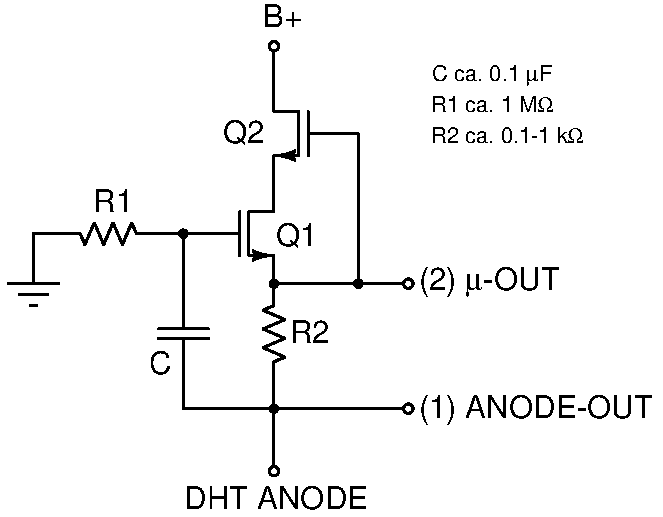
\includegraphics[width=0.5\textwidth]{activeload_concept.pdf}
\caption{Simplified circuit of the active load (AC-coupled CCS).}
\figlabel{activeload_concept}
\end{center}
\end{figure}

In the audio/AC domain, the gate of Q1 is connected to the anode through capacitor C. Q1 mirrors any AC variation in the anode voltage from its gate to its source pin. This configuration maintains a constant voltage between the source of Q1 and the DHT anode, thereby ensuring a constant current through R2. If the headphone stator is driven directly by the DHT anode (output 1 in \figr{activeload_concept}), this current is shared between the DHT and the stator. Consequently, the current flowing through the DHT will exhibit slight variations in response to the AC current consumed by the stator. These variations are typically less than \SI{4}{mA}\cite{osdeha_p8}, which is significantly smaller than the DC bias current. As a result, the load line seen by the DHT anode will closely resemble the one shown in \figr{801A_curves}, although it may not be perfectly flat. Alternatively, the stator can be connected to the $\mu$-output (output 2 in \figr{activeload_concept}) instead of taking the audio output directly from the DHT anode. In this $\mu$-follower configuration\cite{pimm_ccs,kimmel_mustage}, the stator draws its current directly from Q1 rather than through R2. This restores the constant-current operation of the DHT tube and produces a flat load line as shown in \figr{801A_curves}. The value of R2 is typically chosen as a compromise between maximizing the impedance of the CCS load and minimizing the voltage drop (and heat dissipation) across R2\cite{muresistorvalue}.

In the DC domain, the gate of FET Q1 is grounded through R1, fixing the source pin at $-V_{\rm GS,0}$. This arrangement biases the anode at a slightly negative DC voltage determined by $V_{\rm GS,0}$ and the DC voltage drop across R2. As a result, the amplifier outputs maintain a stable DC voltage, effectively compensating for any thermal drift or aging of the DHT tubes.


\subsection{Input Stage}\seclabel{inputstage}

The primary function of the input stage is to amplify the balanced input signal ($2 \times \SI{3.5}{V}$ peak-to-peak) to a level sufficient to drive the DHT grids ($2 \times \SI{86}{V}$ peak-to-peak). This requires a voltage gain of $86 / 3.5 = 25\times$.

Following the lines of the output stage, the differential input stage is designed as long-tailed pair (LTP)\cite{valvewizard_LTP} utilizing tubes with triode characteristics. To maximize the linearity and voltage gain of the LTP, the ``tail'' is configured as a constant-current source (CCS), as illustrated in \figr{IPS_concept}.

\begin{figure}
\begin{center}
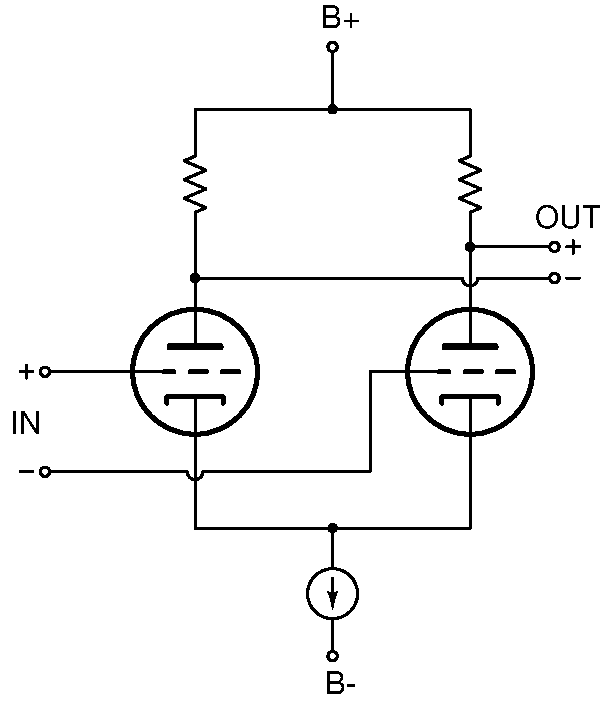
\includegraphics[width=0.6\textwidth]{IPS_concept.pdf}
\caption{Simplified circuit of the input stage.}
\figlabel{IPS_concept}
\end{center}
\end{figure}

A triode-connected 6E5P tube provides suitable gain and exhibits very linear amplification\cite{bartola_thdbenchmark,osdeha_p33}. Each 6E5P is biased at \SI{10}{mA} with an anode-to-cathode voltage of \SI{170}{V} and a \SI{25}{k\Ohm} load resistor, providing more than \SI{\pm100}{V} of anode AC swing (\figr{6E5P_curves}).

\begin{figure}
\begin{center}
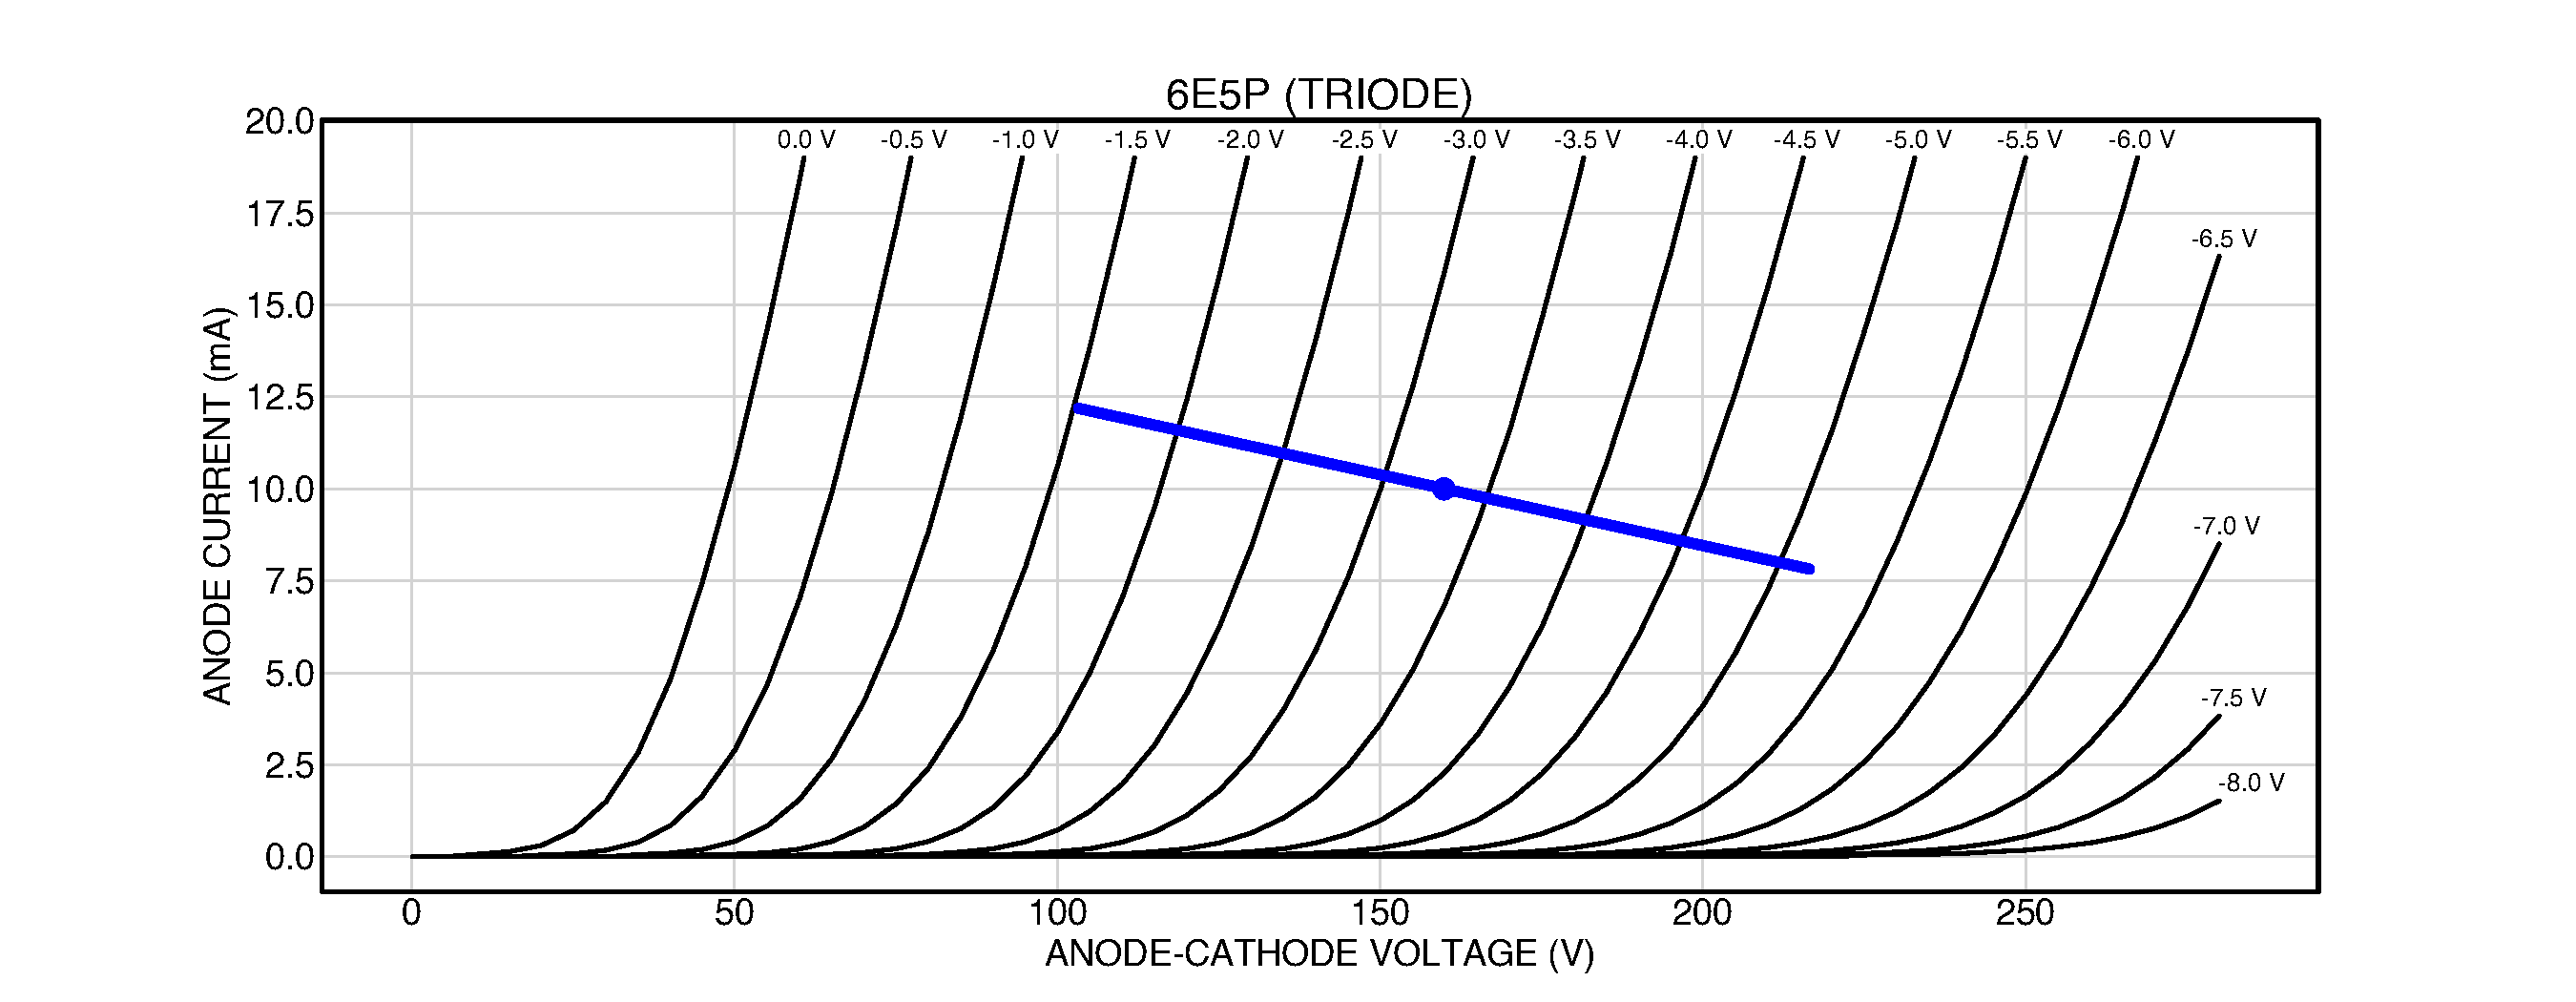
\includegraphics[width=0.8\textwidth]{6E5P_curves.pdf}
\caption{Characteristic curves of a triode-connected 6E5P tube, showing a \SI{25}{k\Ohm} load line with DC bias at \SI{170}{V} and \SI{10}{mA}.}
\figlabel{6E5P_curves}
\end{center}
\end{figure}

The LTP input stage is capacitor-coupled to the grids of the output DHTs. A properly chosen capacitor does not introduce measurable distortion to the audio signal\cite{bateman_caps_distortion}, provided there is no significant current flow across it\cite{aiken_farting_out}. To ensure stable biasing, the DHT grids are driven by FETs configured as source followers. The DC bias voltage for the DHT output tubes is applied to the gates of these FETs, ensuring stable operation even when the DHT grids are driven into grid current.


\section{Power Supplies}

\subsection{High-Voltage Supplies (B+, B-, B2-)}
The amplifier's input and output stages operate on a bipolar high-voltage supply (B+ and B- rails). Additionally, the DHT grids require a bias voltage more negative than B-, necessitating an additional B2- supply. All three high-voltage supplies utilize the same circuit design to deliver clean and stable voltage outputs (\figr{HV_PSU_simple}). The circuits are deliberately designed without feedback-based voltage regulation, as such feedback loops are often associated with sound degradation. A full-wave rectifier and smoothing capacitor (C1) generate a raw DC voltage. This raw supply feeds a current source that injects a small, constant current into R1 and C1. Once C1 is fully charged after startup, R1 develops a constant voltage drop, which serves as a reference mirrored to the voltage output across the DC+ and DC- terminals. For the B+ supply, the DC- output is referenced to GND, while the B- and B2- supplies have their DC+ terminals at GND.

\begin{figure}
\begin{center}
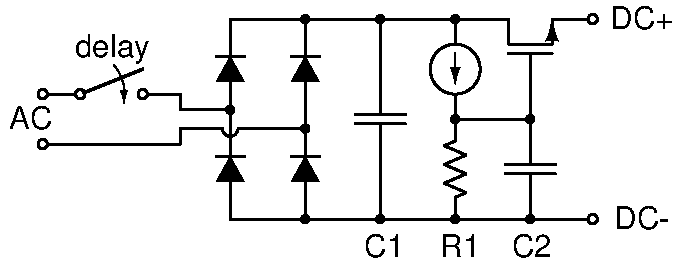
\includegraphics[width=0.5\textwidth]{HV_PSU_concept.pdf}
\caption{Simplified circuit of the high-voltage power supplies.}
\figlabel{HV_PSU_simple}
\end{center}
\end{figure}

To prevent audio noise during startup and reduce stress on the tubes, the high-voltage supplies are activated only after the tubes have warmed up for a few seconds. This delay is implemented using a relay switch controlled by a timer triggered by the heater supply.

\subsection{Diaphragm Bias Voltage}
High-performance electrostatic headphones typically require a \SI{580}{V} DC bias voltage for the diaphragm. The current output of the bias voltage supply is negligible. A charge pump riding on the B+ rail and its AC supply is used to charge a string of capacitors, with their voltage limited to the intended bias level by a string of Zener diodes in parallel to the capacitors. It is crucial to maintain the \emph{charge} on the diaphragm, rather than the diaphragm voltage. To this end, a high-ohmic current-limiting resistor is inserted in the output of the bias supply.

\subsection{Heater Supply for the Input-Stage Tubes}
The heaters of the input-stage tubes are powered by a clean DC voltage to prevent crosstalk of hum or noise from the heater supply into the audio signal. This DC supply is implemented using a standard three-pin voltage regulator chip.

\subsection{DHT Filament Supply}
Like the input-stage heaters, the DHT filaments are powered by DC. However, in DHTs, the filament also serves as the cathode and is part of the audio circuit. During audio playback, a small signal voltage develops across the filament terminals. To prevent the DC filament supply from interfering with this AC signal, it is preferable to control the filament supply current rather than the voltage. This is accomplished using the Coleman Regulator\cite{ColemanDTHFilReg}. The OSDEHA utilizes four Coleman Regulator V9 boards (one per DHT). In each amplifier channel, a single raw DC supply can power a pair of V9 boards.


\section{Putting the Pieces Together}

\figr{system_overview} provides an overview of the various OSDEHA units and their interconnections. The units are distributed across two chassis: one for the power supply and another for the amplifier.

\begin{figure}
\begin{center}
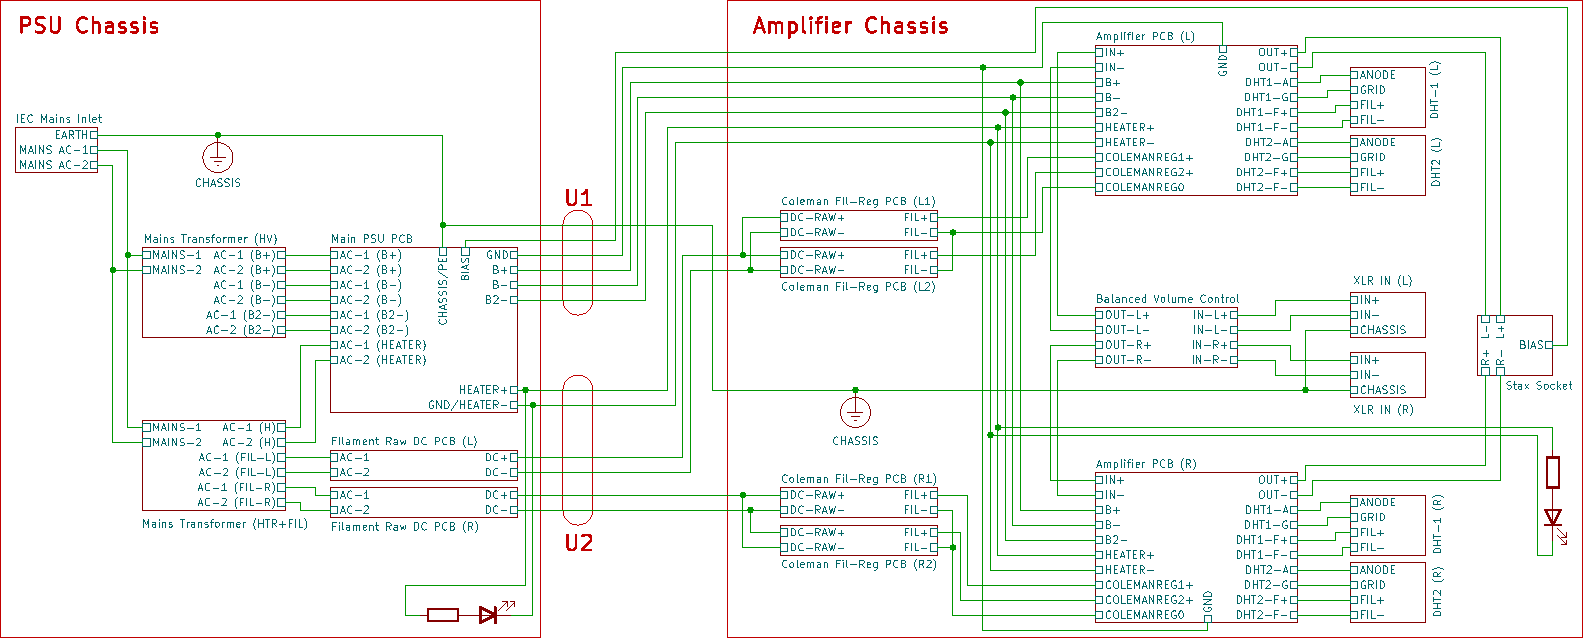
\includegraphics[angle=90,height=0.9\textheight]{system_boards_overview.pdf}
\caption{Overview of the OSDEHA units and their connections (see text).}
\figlabel{system_overview}
\end{center}
\end{figure}

Power-supply chassis:
\begin{itemize}
\item IEC mains inlet with a power switch and mains fuses
\item Two mains transformers
\item Main power-supply board providing stabilized DC voltages for B+, B-, B2-, diaphragm bias, and the heaters of the input-stage tubes
\item Two boards supplying raw DC to the Coleman DHT filament regulators
\end{itemize}

Amplifier chassis:
\begin{itemize}
\item Two amplifier main boards (left and right channels)
\item Four DHT power tubes (two per channel)
\item Four Coleman DHT filament regulators
\item Two XLR audio input sockets
\item Stereo balanced volume control
\item Stax headphone output socket
\end{itemize}

The two chassis are interconnected by two umbilical cables, U1 and U2. U1 carries the high-voltage, low-current supplies (B+, B-, B2-, GND) and provides the chassis-to-earth connection. U2 carries the low-voltage, high-current supplies for the heaters of the input-stage tubes and the Coleman DHT filament regulators.


\section{Mechanical construction}

HEATSINKS, CHASSIS, ETC.

UMBILICALS BETWEEN PSU AND AMP CHASSIS in \figr{power_pinouts}.

\begin{figure}
\begin{center}
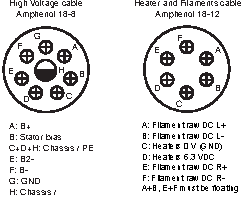
\includegraphics[width=0.5\textwidth]{PSU_CONNECTORS_PINOUTS}
\caption{Pinout of the power umbilical connections between the power supply and amplifier chassis.}
\figlabel{power_pinouts}
\end{center}
\end{figure}


\section{Build Notes, Bring-Up, and Initial Adjustments}

The process of building, testing, and adjusting the OSDEHA is best carried out step by step, as outlined below. Use a variac to gradually ramp up mains power while bringing up the circuits. Turn off the power supply and set the variac output to zero before each step. Before working on the circuits, always ensure that no dangerous voltages remain present (e.g., all capacitors are discharged, and the mains cable is disconnected).

\subsection{Power Supply}
\begin{itemize}
\item Assemble the power-supply chassis and boards. Install the boards, sockets, and transformers in the power-supply chassis. Wire the primary windings of the transformers to the mains inlet and power switch in the chassis. Wire the power supply outputs to the umbilical sockets.
\item Confirm proper connection of all metal parts of the power-supply chassis to mains earth.
\item Wire the transformer secondaries for the heater supply. Switch on the power supply and gradually ramp up mains power using the variac. Confirm that the heater supply functions as expected. Verify the operation of the high-voltage delay relay.
\item Wire the transformer secondaries for the DHT raw-DC filament supplies. Switch on the power supply and gradually ramp up the variac to confirm that the raw-DC supplies function correctly.
\item Wire the transformer secondaries for the high-voltage supplies and install dummy resistors at their outputs. Switch on the power supply and gradually ramp up the variac. Confirm and adjust the high-voltage output levels as needed. Verify the diaphragm bias voltage output (note: the internal resistance of the voltmeter will load the bias output, resulting in a lower voltage reading). Remove the dummy resistors from the high-voltage supplies.
\end{itemize}

\subsection{Amplifier Input Stage}
\begin{itemize}
\item Determine the CCS sense-resistor values that yield the targeted bias currents for the CCSs with the specific DN2540 parts used in the input LTP tail and in the DHT grid drivers (\figr{CCS_Rsense_jig}).
\item Assemble the amplifier chassis, amplifier boards, and Coleman filament regulators. Install the boards and sockets in the amplifier chassis. Install the input-stage tubes, but do \emph{not} install the DHT tubes of the output stages yet. Do \emph{not} yet wire the umbilical sockets to the boards.
\item Install the umbilical cables between the power supply and the amplifier chassis. Wire the amplifier chassis to the earth pins of the umbilical socket. Verify the electrical connection of all metal parts of the amplifier chassis to the power-supply chassis and mains earth. Make sure the XLR pins~1 are connected to the chassis.
\item Wire the heater supply from the umbilical socket to the amplifier boards. Switch on the power supply and gradually ramp up the variac. Verify functioning of the heaters in the input-stage tubes.
\item Wire the high-voltage supplies (B+, B-, B2-) and GND from the umbilical socket to the amplifier boards. Switch on the power supply and gradually ramp up the variac. Verify the correct DC bias of the input-stage tubes (plate voltages and currents) and the DC bias currents of the buffer stages.
\item Wire the audio inputs from the XLR sockets to the volume control and to the amplifier boards. Apply an AC test signal to the XLR sockets and trace the signal path through the circuit, and verify correct output from the buffer stage to the grid pins on the DHT sockets.
\end{itemize}

\begin{figure}
\begin{center}
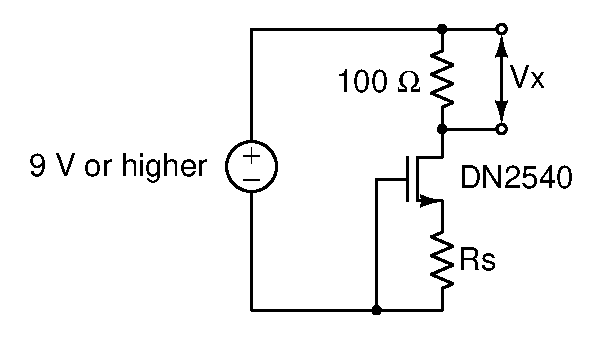
\includegraphics[width=0.38\textwidth]{CCS_Rsense_circuit}
\caption{Circuit to determine the sense-resistor value $R_{\rm s}$ that yields the desired CCS current for a given DN2540 part. Adjust the $R_{\rm s}$ value until the voltage drop $V_{\rm x}$ across the \SI{100}{\Ohm} resistor corresponds to the desired current.}
\figlabel{CCS_Rsense_jig}
\end{center}
\end{figure}


\subsection{Amplifier Output Stage}
\begin{itemize}
\item With the output tubes still not installed in the amplifier, adjust the grid bias voltage to the most negative value.
\item Disconnect the high-voltage supplies from the amplifier boards. Wire the DHT filament supplies from the umbilical socket to the Coleman filament regulators and to the amplifier boards. Install the DHT output tubes. Switch on the power supply and gradually ramp up the variac while monitoring the DHT filament voltages and paying attention to not exceed the datasheet value. Adjust the filament voltage to the target value. Allow the tubes to warm up and readjust the filament voltage as needed.
\item Reconnect the high-voltage supplies to the amplifier boards, switch on the power supply and gradually ramp up the variac. Monitor the DC bias currents of each output tube by measuring the voltage drop across the mu-resistors. Adjust the DC grid bias until the desired DC bias points are attained. Allow the amplifier to warm up and readjust the DC bias as necessary. Also monitor the filament voltages during warmup and adjust if needed.
\item Apply an AC test signal to the amplifier inputs and verify correct outputs from the amplifier.

\end{itemize}


\section{Specifications and Test Results}

TESTS AND MEASUREMENTS

OUTPUT BEFORE CLIPPING

FREUQNECY RESPONSE

DISTORTION MEASUREMENTS (THD, IMD, SPECTRA)


\section{Parts List}

The details of most electronic components used in the OSDEHA circuits (tubes, semiconductors, resistors, capacitors) are provided in the KiCad files located in the {\tt kicad/} directory.\cite{osdeha_github} Additional parts, such as chassis, mounting hardware, and connectors, are listed below.

{\footnotesize \csvautobooktabular[separator=tab]{partslist.txt}}

\clearpage
\section{License information} \seclabel{license}
Copyright Matthias Brennwald 2024.                                                    

The OSDEHA is Open Hardware and is licensed under the CERN-OHL-S v2 or any later version.

You may redistribute and modify this source and make products using it under the terms of the CERN-OHL-S v2 (\url{https://ohwr.org/cern_ohl_s_v2.txt}).

This source is distributed WITHOUT ANY EXPRESS OR IMPLIED WARRANTY, INCLUDING OF MERCHANTABILITY, SATISFACTORY QUALITY AND FITNESS FOR A PARTICULAR PURPOSE. Please see the CERN-OHL-S v2 for applicable conditions.

Source location: \url{https://github.com/mbrennwa/OSDEHA}

As per CERN-OHL-S v2 section 4, should You produce hardware based on this source, You must where practicable maintain the Source Location visible on the external case of the OSDEHA or other products you make using this source.            


% list of references
\clearpage
\bibliographystyle{unsrt}
\bibliography{OSDEHA_documentation}


\end{document}
